\chapter{Theoretische Grundlagen}
\thispagestyle{fancy}
\textbf{Hier fehlt noch eine generelle Einleitung zum Kapitel}

\section{Struktur der Anwendung}
In diesem Abschnitt soll zunächst die generelle Struktur der Anwendung definiert werden. Weite Teile der Struktur können dabei aus dem Praxisprojekt übernommen werden. Im Praxisprojekt wurden die folgenden Themengebiete behandelt:

\begin{itemize}
  \item Typographie
  \item Layout \& Struktur
  \item Whitespace
  \item Farben
  \item Bilder
  \item Interaktive Elemente
\end{itemize}

Nach einer erneuten evaluation der Ergebnisse des Praxisprojektes konnten die in der Abschlussarbeit zu behandelnden Themengebiete auf zunächst drei eingegrenzt werden (der Bereich \textit{Layout \& Struktur} wurde dabei in \textit{Layout \& Grids} umbenannt):

\begin{itemize}
  \item Typographie
  \item Layout \& Grids
  \item Farben
\end{itemize}

Diese Abgrenzung begründet sich auf verschiedene Weisen. Im Fall des Bereiches \textit{Whitespace} konnte im Rahmen des Praxisprojektes kein zufriedenstellendes Konzept erarbeitet werden, wodurch sich dieser Bereich per se nicht für eine Umsetzung eignet. Weiterhin muss es Ziel dieser Arbeit sein, am Schluss eine vollständige Anwendung zu erhalten. Um dieses Ziel im zeitlichen Rahmen erreichen zu können mussten weitere Themengebiete vernachlässigt werden. Hier boten sich die Bereiche \textit{Bilder} und \textit{Interaktive Elemente} an, da diese für die gestalterische Grundqualität eine vergleichsweise niedrige Rolle spielen. \textbf{NOTE: Vielleicht muss das hier noch belegt werden, wie ein Brötchen}. Diese Bereiche wurden aber ausreichend konzeptioniert und bieten sich als erste Erweiterungen für die Anwendung nach beenden der Arbeit an.

Außerdem müssen für die Anwendung jeweils ein nutzerfreundlicher Einstieg und Ausstieg gefunden werden. Diese wurden im Praxisprojekt nicht explizit ausgearbeitet und fallen somit auch Konzeptionell in den Bereich der Abschlussarbeit und werden später in diesem Kapitel behandelt.

Die finale Struktur der Anwendung für den Rahmen dieser Arbeit sieht also wie folgt aus:

\begin{itemize}
  \item Einstieg
  \item Typographie
  \item Layout \& Grids
  \item Farben
  \item Ausstieg
\end{itemize}

\subsection{Einstieg in die Anwendung}
Bereits im Praxisprojekt wurde festgestellt, dass es sinnvoll ist, das Zielmedium des Nutzers zu kennen. Mit Blick auf die Zielgruppe wurden hier drei mögliche Bereiche definiert: Native App, Website und Textdokument. \textbf{NOTE: Hier verweis auf Untersuchung im PP}. Diese Bereiche können jedoch auch in sich verschiedene Eigenarten aufweisen, so kann ein Textdokument beispielsweise für das Lesen an einem Bildschirm oder das Lesen in gedruckter Form entworfen werden. Eine komplette Auflistung der möglichen Bereiche oder \textit{scopes} der Anwendung findet sich in Abbildung \ref{fig:intro} auf Seite \pageref{fig:intro}.

\begin{figure}[h]
    \centering
    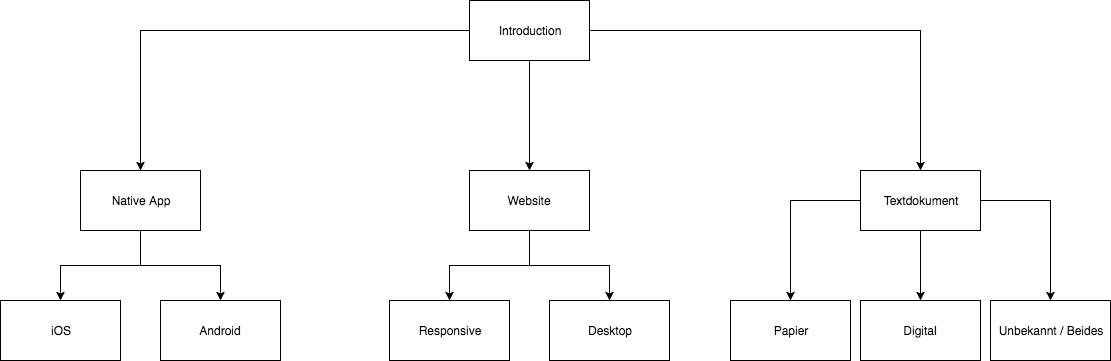
\includegraphics[width=1\textwidth]{images/ablauf_intro.png}
    \caption{Mögliche Entscheidungen im Einstieg der Anwendung}
    \label{fig:intro}
\end{figure}

Obwohl die Abgrenzung der Bereiche für die hier definierte Zielgruppe ausreichend ist, lassen sich bereits jetzt einige Stellen erkennen, die bei einer möglichen späteren Erweiterung der Zielgruppe überarbeitet werden müsste. Vorrangig betrifft das den Bereich \textit{Website}. Hier ist die vorhandene Unterteilung in \textit{Responnsive} und \textit{Desktop} für ein Echtwelt-Szenario unter Umständen zu allgemein gehalten.

Um den kognitiven Aufwand \textbf{Beleg} für den Nutzer möglichst gering zu halten, bietet es sich an, ihn Schrittweise durch das Festlegen des für ihn passenden Bereiches zu führen.

\subsection{Ergebnisse der Benutzung}
Eines der Ziele der Anwendung ist es, dem Nutzer währen der Nutzung auf interaktive weise Wissen zu vermitteln. Da der Nutzer jedoch während der Nutzung auch konkrete Ergebnisse erarbeitet wäre es hier kontraproduktiv, ihm diese Ergebnisse nicht am Ende der Anwendung noch einmal explizit zukommen zu lassen (zusätzlich zum implizit gesammelten Wissen).

Dieser Bereich wurde im Rahmen des Praxisprojektes nicht ausdefiniert, ist aber für die Wahrnehmung der Anwendung als fertiges Produkt durchaus wichtig. Eine gute Darstellung der Ergebnisse des Nutzers definieren einen ausschlaggebenden Teil der Nutzungserfahrung.
Hier sollen also mögliche Darstellungen der Ergebnisse diskutiert werden und vorrangig zwei Fragen beantwortet werden:
\begin{enumerate}
  \item Welche Darstellung der Ergebnisse ist für den Nutzer am Vorteilhaftesten?
  \item Welche Darstellung bietet den besten Kompromiss aus Umsetzbarkeit und Mehrwert für den Nutzer?
\end{enumerate}

Die einfachste Darstellung ist eine Transistente Darstellung innerhalb der Anwendung am Ende der Verwendung. Eine Darstellung ist wegen der Haltung der ermittelten Werte im Redux-Store der Anwendung einfach. Obwohl einfach umzusetzen, ist diese Lösung nicht optimal: Nachdem der Nutzer die Anwendung schließt sind die erarbeiteten Daten verloren, da diese nicht persistent gespeichert werden.

Ein naheliegender Schritt ist also eine Persitierung des Wissens für den Nutzer. Hier bieten sich verschiedene Möglichkeiten, wie zum Beispiel das Speichern in Cookies oder das Entwicklen eines Backends, an. Ein Kompromiss zwischen Usability und Entwicklungsaufwand wäre hierbei die persistieren des Wissen in einer herunterladbarer Datei, beispielsweise als PDF.

Eine weitere Frage beschäftigt sich mit dem Aufbau dieser Datei. Auch hier wäre der einfachste Ansatz, die Ergebnisse des Nutzers einfach aufzulisten. Optimal wäre eine Aufbereitung der Daten, sodass der Nutzer diese möglichst ohne weitere Manipulation in seinen Workflow übernehmen kann. Obwohl das Zielmedium des Nutzers bekannt ist, zeigt sich hier das Problem, dass innerhalb dieser Zielmedien weiterhin verschieden Tools verwendet werden können, die eine unterschiedliche Aufbereitung der Daten erfordern.
Beispielsweise kann bekannt sein, dass der Nutzer eine Webandwendung entwickelt und das Styling für seine texte in CSS vornimmt. Trotzdem kann der Nutzer zum Beispiel verschieden Preprozessoren wie SCSS, SASS oder LESS verwenden, die alle eine unterschiedliche Syntax verwenden.
Es liegt dabei durchaus im Rahmen des Möglichen, diese Informationen vom Nutzer zu erhalten und die Daten entsprechend aufzubereiten, jedoch liegen diese Anforderungen außerhalb des Zeitlichen Rahmens dieser Abschlussarbeit.

Hier wird dem Nutzer daher zunächst eine PDF zur Verfügung gestellt. Ein exemplarischer Aufbau kann ABB. XYZ entnommen werden.

\section{Diskussion verfügbarer Technologien}
Im Nachfolgenden Kapitel sollen mögliche Technologien diskutiert werden, die für die Umsetzung der Abschlussarbeit genutzt werden können. Für die Umsetzung einer Webanwendung bieten sich eine Vielzahl von Programmiersprachen und Frameworks an. Diese können durch die geplante Struktur der Anwendung jedoch bereits weiter eingegrenzt werden. Da die Anwendung keine persistente Datenhaltung implementiert und auch keine übermäßig aufwendigen Berechnungen durchgeführt werden müssen, kann auch ein klassisches Client-Server-Modell verzichtet werden.
Aufgrund des hohen Grades der Interaktivität der Anwendung kann außerdem davon ausgegangen werden, dass in jedem Falle auf JavaScript zurück gegriffen werden muss.

In den letzten Jahren wurden viele JavaScript-Frontend-Frameworks veröffentlicht, die genau auf die Anforderung der gestiegenen Interaktivität im Browser reagieren.
Im Praxisprojekt wurde bereits versucht, den Proof of Concept nur mithilfe des Frameworks jQuery umzusetzen. Hier wurde schnell deutlich, dass die Komplexität der Anwendung den Rahmen von jQuery übersteigt.

Im folgenden sollen also einige der bekanntesten JavaScript-Frontend-Frameworks verglichen werden. Die Auswahl dieser Frameworks erfolgt nach Beliebtheit auf GitHub.com. Weiterhin wurden Frameworks ausgeschlossen, die ein komplettes MCV-Pattern implementieren, da zum aktuellen Stand dieser Anwendung keine Models angemacht sind.

\subsection{Vue.js}
Bei der Textgestaltung und automatischen Änderung von Abbildungsnummern, Querverweisen,
Seitenzahlen, Gliederungen, Literaturhinweisen etc. bietet sich der Rückgriff
auf moderne Textverarbeitungsprogramme an. Nutzen Sie diese zur besseren Lesbarkeit
und Strukturierung des Textes, aber vermeiden Sie überflüssige Spielereien. Da
besonders bei Textdokumenten mit eingebundenen Objekten wie Bildern, Formeln

\subsection{Angular.js}
Bei der Textgestaltung und automatischen Änderung von Abbildungsnummern, Querverweisen,
Seitenzahlen, Gliederungen, Literaturhinweisen etc. bietet sich der Rückgriff
auf moderne Textverarbeitungsprogramme an. Nutzen Sie diese zur besseren Lesbarkeit
und Strukturierung des Textes, aber vermeiden Sie überflüssige Spielereien. Da
besonders bei Textdokumenten mit eingebundenen Objekten wie Bildern, Formeln

\subsection{React.js}
Bei der Textgestaltung und automatischen Änderung von Abbildungsnummern, Querverweisen,
Seitenzahlen, Gliederungen, Literaturhinweisen etc. bietet sich der Rückgriff
auf moderne Textverarbeitungsprogramme an. Nutzen Sie diese zur besseren Lesbarkeit
und Strukturierung des Textes, aber vermeiden Sie überflüssige Spielereien. Da
besonders bei Textdokumenten mit eingebundenen Objekten wie Bildern, Formeln

\section{Einstieg in React.js}
Bei der Textgestaltung und automatischen Änderung von Abbildungsnummern, Querverweisen,
Seitenzahlen, Gliederungen, Literaturhinweisen etc. bietet sich der Rückgriff
auf moderne Textverarbeitungsprogramme an. Nutzen Sie diese zur besseren Lesbarkeit
und Strukturierung des Textes, aber vermeiden Sie überflüssige Spielereien. Da
besonders bei Textdokumenten mit eingebundenen Objekten wie Bildern, Formeln

\subsection{Komponenten}
Der Komponentenbasierte Aufbau ist eines der Hauptaugenmerke von React.js. Komponenten werden auf der offiziellen React.sj-Website \footnotemark als der wichtigsten Merkmale aufgeführt und Gackenheimer \cite[S. 28]{Gackenheimer201509} nennt sie einen der Hauptbestandteile einer React-Anwendung. \\
Dieser Abschnitt beschäftigt sich mit dem Aufbau, der Verwendung, den verschiedenen Formen und den Besonderheiten von Komponenten in React. \\
Natürlich kann und soll es nicht Ziel sein, einen umfassenden überblick über alle Informationen zu geben, die mit Komponenten in React in Verbindung stehen. Daher soll im Folgenden vorrangig auf in der Umsetzung als am relevantesten empfundene Aspekte eingegangen werden.
\footnotetext{https://facebook.github.io/react/}


\subsubsection{Was ist eine Komponente?}
Bevor auf die Besonderheiten von Komponenten in React.js eingegangen wird, soll im Folgenden kurz ein Überblick über das Konzept der Komponente an sich gegeben werden.

Das Oxford Dictionary definiert eine Komponente als

\begin{quote}
  A part or element of a larger whole […]
\end{quote}

Gerade im Bezug auf Softwareentwicklung werden Komponenten aber noch einige weitere Eigenschaften zugeschrieben. So schreiben \cite{Szyperski200211} über Komponenten in der Softwareentwicklung:


\begin{quote}
  One thing can be stated with certainty: components are for composition. […] Composition enables prefabricated “things” to be reused by rearranging them in ever-new composites.
\end{quote}

Das Hauptaugenmerk bei der Entwicklung einer Komponente in der Softwareentwicklung sollte also auf der Möglichkeit der Wiederverwendbarkeit innerhalb der Anwendung liegen. Dabei sollte der Ort für die Wiederverwendung keine Rolle spielen. Eine Komponente sollte also unabhängig von ihrer Umgebung die gleichen Ergebnisse liefern \cite{de2001interface}:


\begin{quote}
  It does not constrain the environment but describes the behavior of the component in an arbitrary environment: “for all inputs x and y, if y $\neq$ 0, then the output is z = x/y“
\end{quote}

\subsubsection{Komponenten in React.js}
Bei der Textgestaltung und automatischen Änderung von Abbildungsnummern, Querverweisen,
Seitenzahlen, Gliederungen, Literaturhinweisen etc. bietet sich der Rückgriff
auf moderne Textverarbeitungsprogramme an. Nutzen Sie diese zur besseren Lesbarkeit
und Strukturierung des Textes, aber vermeiden Sie überflüssige Spielereien. Da
besonders bei Textdokumenten mit eingebundenen Objekten wie Bildern, Formeln

\subsubsection{Stateful \& Stateless}
Komponenten in React.js können entweder Stateful oder Stateless sein. Wie der Name bereits vermuten lässt, haben diese Komponenten entweder  einen state, oder nicht.\\
Der state in React.js beschreibt den Zustand eine Komponente. Hier findet sich auch eines der Hauptfeatures von React.js: Ändert sich der state einer Komponente, so wird diese Komponente neu gerendert, also auch das User Interface aktualisiert um den neuen Zustand darzustellen. Der state kann (und sollte) dabei durch das Aufrufen der Funktion \verb|setState()| geändert werden. Das nachfolgende Codebeispiel zeigt eine simple Komponente, die clicks auf einen Button zählt:

\begin{lstlisting}
  class ClickCounter extends React.Component{
  	constructor(props) {
  		super(props)

  		this.state = {clicks: 0}
  	}

    handleClick() {
  		this.setState((prevState) => {
    			return {clicks: prevState.clicks + 1};
  		});
  	}

  	render() {
  		return (
  			<button onClick={this.handleClick}>Click me!</button>
  			{this.state.clicks}
  		)
  	}
  }
\end{lstlisting}

Hier passiert folgendes: Im Konstruktor der Komponente (der nur ein mal, beim initialen rendern aufgerufen wird) wird die initiale Anzahl der Clicks im state auf 0 gesetzt.
Die Komponente rendert ein \verb|<buttton>| element und die Anzahl der gezahlten Klicks. Wird der Button geklickt, wird die Funktion \verb|handleClick()| in der Komponente aufgerufen. Diese Funktion erhöht die Anzahl der Klicks im state um eins. Durch den aktualisierten state wird auch die Komponente neu gerendert, so dass nun auch die neue Klickzahl angezeigt wird. \\

Die Komponente im obigen Beispiel ist also Stateful. Wie schon früher in diesem Kapitel erwähnt, ist es aber Ziel der Komponentenbasierten Softwareentwicklung, wiederverwendbare Komponenten zu schreiben.\\
Diese Komponente ließe sich an jeder Stelle der Anwendung wiederverwenden, an der Klicks über einen Button gezählt werden müssen, jedoch ist die Wahrscheinlichkeit hoch, dass diese Anwendungsfall eher selten vorkommt. Außerdem ist die Wahrscheinlichkeit recht hoch, dass ein Button oder ein Element zur Darstellung von Werten in der Anwendung häufiger verwendet werden (natürlich würde eine einfache Darstellung wie im obigen Beispiel kein Sinn ergeben, für dieses Beispiel soll daher eine komplexere Darstellung der Daten angenommen werde, beispielsweise durch eine Progress-Bar).
Eigentlich liegen hier also drei Komponenten vor: Eine Komponente, die Logik enthält und zwei weitere, die lediglich Daten darstellen, somit also stateless sind.\\

Mit dem release von React 0.14 (https://facebook.github.io/react/blog/2015/09/10/react-v0.14-rc1.html) wurde eine simplifizierte Schreibweise für stateless components eingeführt. Die beiden Komponente aus dem Beispiel könnten somit wie folgt definiert werden:

\begin{lstlisting}
  export default function Button = (props) => {
  	return (
  		<button onClick={props.onClick}>Click me!</button>
  	)
  }
\end{lstlisting}

und

\begin{lstlisting}
  export default function ValueDisplay = (props) => {
  	return (
  		<div>{props.value}</div>
  	)
  }
\end{lstlisting}

Die Werte für diese Komponenten werden ihnen in der Oberkomponente als \verb|props| übergeben:

\begin{lstlisting}
  class ClickCounter extends React.Component{
  	constructor(props) {
  		super(props)

  		this.state = {clicks: 0}
  	}

    handleClick() {
  		this.setState((prevState) => {
    			return {clicks: prevState.clicks + 1};
  		});
  	}

  	render() {
  		return (
  			<Button onClick={this.handleClick} />
  			<ValueDisplay value={this.state.clicks} />
  		)
  	}
  }
\end{lstlisting}

Ziel muss es also sein, so viele Komponenten wie möglich so klein wie möglich, optimaler Weise mit nur einer einzigen Aufgabe zu schreiben, um die Wiederverwendbarkeit zu erhöhen.

\subsection{JSX}
Bei der Textgestaltung und automatischen Änderung von Abbildungsnummern, Querverweisen,
Seitenzahlen, Gliederungen, Literaturhinweisen etc. bietet sich der Rückgriff
auf moderne Textverarbeitungsprogramme an. Nutzen Sie diese zur besseren Lesbarkeit
und Strukturierung des Textes, aber vermeiden Sie überflüssige Spielereien. Da
besonders bei Textdokumenten mit eingebundenen Objekten wie Bildern, Formeln

\subsection{Weitergabe von Daten}
Bei der Textgestaltung und automatischen Änderung von Abbildungsnummern, Querverweisen,
Seitenzahlen, Gliederungen, Literaturhinweisen etc. bietet sich der Rückgriff
auf moderne Textverarbeitungsprogramme an. Nutzen Sie diese zur besseren Lesbarkeit
und Strukturierung des Textes, aber vermeiden Sie überflüssige Spielereien. Da
besonders bei Textdokumenten mit eingebundenen Objekten wie Bildern, Formeln





\section{Technologie-Stack}
Bei der Textgestaltung und automatischen Änderung von Abbildungsnummern, Querverweisen,
Seitenzahlen, Gliederungen, Literaturhinweisen etc. bietet sich der Rückgriff
auf moderne Textverarbeitungsprogramme an. Nutzen Sie diese zur besseren Lesbarkeit
und Strukturierung des Textes, aber vermeiden Sie überflüssige Spielereien. Da
besonders bei Textdokumenten mit eingebundenen Objekten wie Bildern, Formeln

\section{Gestaltung}
Bei der Textgestaltung und automatischen Änderung von Abbildungsnummern, Querverweisen,
Seitenzahlen, Gliederungen, Literaturhinweisen etc. bietet sich der Rückgriff
auf moderne Textverarbeitungsprogramme an. Nutzen Sie diese zur besseren Lesbarkeit
und Strukturierung des Textes, aber vermeiden Sie überflüssige Spielereien. Da
besonders bei Textdokumenten mit eingebundenen Objekten wie Bildern, Formeln
